\chapter{$\bholomorphic{\disk}$ como álgebra de Banach}
\label{cap:banach}

En este capítulo vamos a presentar algunos conceptos y resultados generales sobre álgebras de Banach, particularizando el estudio en el álgebra de las funciones holomorfas acotadas en el disco unidad, $\bholomorphic{\disk}$. En este caso, el espectro (el espacio de homomorfismos no nulos entre $\bholomorphic{\disk}$ y $\complex$) se descompone como unión disjunta de las fibras sobre los puntos del disco cerrado. A través de las fibras se estudia el comportamiento de los elementos de $\bholomorphic{\disk}$ en los puntos del borde, tanto cuando la función puede extenderse con continuidad como en el caso más interesante, de puntos singulares en el borde. En este análisis recuperamos, bajo la nueva perspectiva, ejemplos concretos que se estudiaron en capítulos previos. \\

\section{Álgebra de Banach}

\begin{definition}
    Un espacio vectorial complejo $X$, dotado de una norma $\norm{\cdot}$ se denomina espacio de Banach si es completo.
\end{definition}

\medskip

En nuestro caso particular, $\bholomorphic{\disk}$ es un espacio vectorial complejo, que dotado con la norma infinito
\begin{equation*}
    \norminf{f} = \sup_{\abs{z} < 1} \abs{f(z)},
\end{equation*}
es normado y completo sobre $\complex$ puesto que el límite uniforme sobre compactos de una sucesión de funciones holomorfas es una función holomorfa. Atendiendo a la definición anterior, decimos que  $(\bholomorphic{\disk}, \norminf{\cdot})$ es un espacio de Banach. \\

\begin{definition}
    Decimos que un álgebra $B$, dotada de una norma $\norm{\cdot}$ es un álgebra de Banach si como espacio normado $(B, \norm{\cdot})$ es un espacio de Banach y, además, para el producto satisface:
    \begin{equation*}
        \forall x, y \in B: \, \norm{x \cdot y} \leq \norm{x} \cdot \norm{y}.
    \end{equation*}
\end{definition}

\medskip

De nuevo, podemos ver $\bholomorphic{\disk}$ como un álgebra, con las operaciones naturales. En efecto, si $f, g \in \bholomorphic{\disk}$ y $\alpha, \beta \in \complex$, entonces
\begin{equation*}
    \begin{split}
        & \alpha f + \beta g \in \bholomorphic{\disk} \\
        & fg \in \bholomorphic{\disk}.
    \end{split}
\end{equation*}

Así, $\bholomorphic{\disk}$ es un álgebra de Banach conmutativa (con la función constante 1 como elemento unidad) puesto que es un álgebra conmutativa y un espacio de Banach cuya norma asociada cumple la siguiente propiedad:
\begin{equation*}
    \forall f, g \in \bholomorphic{\disk}: \, \norminf{f \cdot g} \leq \norminf{f} \cdot \norminf{g}.
\end{equation*}

\section{Espacio dual de un álgebra de Banach}

\begin{definition}
    Sea $B$ un espacio de Banach complejo. Consideramos $B^*$ el espacio de las aplicaciones $\varphi: B \to \complex$ lineales y continuas. $B^*$ es un espacio vectorial y tiene una norma natural dada por:
    \begin{equation*}
        \norm{\varphi} = \sup_{\norm{x} \leq 1} \abs{\varphi(x)}.
    \end{equation*}
    Con esta norma, $B^*$ es un espacio de Banach al que llamamos espacio dual de $B$.
\end{definition}
\medskip

Además de la topología inducida por la norma en el espacio dual $B^*$, vamos a considerar otra topología denominada topología débil-* en $B^*$ que está definida de la siguiente manera. Sea $\varphi_0 \in B^*$, y tomemos una cantidad finita de elementos $x_1, \dots x_n \in B$ y $\varepsilon > 0$. Los entornos de $\varphi_0$ serán los conjuntos que contienen uno de la forma $U$, donde
\begin{equation*}
U = \{ \varphi \in B^*: \abs{\varphi(x_k) - \varphi_0 (x_k)} < \varepsilon, k = 1, \dots, n\}.
\end{equation*}
Un abierto de esta topología será, por tanto, cualquier unión de tales entornos $U$. \\

Esta topología se denota por $\sigma(B^*, B)$. Es la topología más débil de $B^*$ tal que todas las funciones $\varphi \to \varphi(x)$ son continuas de $B^*$ en $\complex$, con $x \in B$. \\ % La topología débil-* es la más débil de $B^*$, es decir, es aquella que tiene el menor número de abiertos.

Un resultado importante de análisis funcional que usaremos en nuestro desarrollo es el Teorema de Alaouglu, que establece la compacidad de la bola unidad cerrada de cualquier espacio dual, cuando se considera dotado de la topología débil-*. Obsérvese que en dimensión infinita, la bola unidad no es compacta en ningún espacio para la topología dada por la norma. \\

\begin{theorem}[de Alaouglu]
    La bola unidad cerrada de $B^*$ es compacto en la topología débil-*.
\end{theorem}

\section{El espectro de un álgebra}

Recordemos que $\varphi: B \to \complex$ es un homomorfismo de álgebras si para todos $x, y \in B$ y $\alpha, \beta \in \complex$ se cumple:
\begin{equation}
    \begin{split}
        & \varphi (\alpha x + \beta y) = \alpha \varphi(x) + \beta \varphi(y) \\
        & \varphi(x \cdot y) = \varphi(x) \cdot \varphi(y).
    \end{split}
\end{equation}

El espectro de $B$, denotado por $\fiber(B)$, es el espacio de los homomorfismos $\varphi: B \to \complex$ no nulos. Observamos que tales homomorfismos verifican que son continuos y $\norm{\varphi} = 1$. \\

Tal y como hemos definido $\fiber(B)$, es un subconjunto del espacio dual $B^*$. De hecho, está contenido en la bola unidad de $B^*$ que, dotada con la topología débil-*, es un compacto. Por lo que al ser $\fiber(B)$ cerrado en $B^*$, este es, a su vez, un espacio Hausdorff compacto. \\

Llegados a este punto queremos asociar cada elemento $x$ de $B$ con una función continua sobre $\fiber(B)$. Para ello vamos a definir la siguiente aplicación
\begin{equation*}
    \begin{split}
        \widehat x:  \fiber(B) & \to  \complex \\
              \varphi \, \, \, & \mapsto  \varphi (x).
    \end{split}
\end{equation*}

Si dotamos a $\fiber(B)$ con la topología débil-*, tenemos que cada $\widehat x$ es una función continua en $\fiber(B)$. Más aún, por definición, la topología débil-* es la topología más débil de $\fiber(B)$ que hace que cada $\widehat x$ sea continua. Así pues, tenemos la siguiente representación a la que se le suele denominar \textbf{transformada de Gelfand}
\begin{equation*}
    x \to \widehat x.
\end{equation*}

La imagen de $B$ bajo este homomorfismo es el álgebra $\widehat B$ de las funciones continuas sobre $\fiber(B)$ que toman valores complejos. Es decir,
\begin{equation*}
    \widehat B = \{\widehat x: \fiber(B) \to  \complex \mid x \in B\}.
\end{equation*}

\medskip

Todos los comentarios que hemos desarrollado anteriormente para un álgebra de Banach cualquiera, siguen siendo ciertos si los particularizamos para el álgebra $\bholomorphic{\disk}$. Así, el espectro, al que vamos a denotar por $\fiber = \fiber (\bholomorphic{\disk})$, será el espacio de los homomorfismos $\phi: \bholomorphic{\disk} \to \complex$ no nulos. \\

La construcción que se ha realizado previamente para $B$, se describe ahora de la siguiente manera. Tenemos la aplicación
\begin{equation*}
    \begin{split}
        \widehat f:  \fiber & \to  \complex \\
                    \phi \, & \mapsto  \phi (f),
    \end{split}
\end{equation*}
para cada $f \in \bholomorphic{\disk}$, donde cada $\widehat f$ es continua sobre el $\fiber$ si dotamos a $\fiber$ con la topología débil-*. Esto da lugar a la representación $f \to \widehat f$. De esta manera, vamos a poder interpretar $\bholomorphic{\disk}$ como el álgebra de las funciones continuas en el espacio compacto $\fiber$. \\

Al espacio $\fiber$ se le suele denominar espacio de ideales maximales de $\bholomorphic{\disk}$. Para cada $\phi \in \fiber$, el núcleo de $\phi$ es un ideal maximal del álgebra $\bholomorphic{\disk}$. Recíprocamente, todo ideal maximal en $\bholomorphic{\disk}$ se corresponde con el núcleo de un homomorfismo en $\fiber$. Más adelante estudiaremos la estructura de este espacio. \\

\begin{comment}
Existe una correspondencia uno a uno entre los homomorfismos $\phi: \bholomorphic{\disk} \to \complex$ y los ideales maximales $M$ en el álgebra $\bholomorphic{\disk}$. Esta correspondencia está definida por $M = \ker (\phi)$. Cada ideal maximal $M$ es cerrado, así que cada homomorfismo $\phi$ es continuo:
\begin{equation*}
    \abs{\phi (x)} \leq \norm{x}.
\end{equation*}
\end{comment}

% Hablar más de la relación de $\fiber$ con los ideales maximales, o también citar un libro de álgebra en el que se hable sobre esto.

En principio, los únicos homomorfismos complejos que se pueden identificar claramente son las evaluaciones en puntos del disco abierto $\disk$. Si $z \in \disk$,
\begin{equation*}
    \begin{split}
        \delta_z: \bholomorphic{\disk} & \to  \complex \\
                   f \, \, \, \, \, \, & \mapsto  f (z).
    \end{split}
\end{equation*}

Así pues, las evaluaciones en puntos del disco abierto son elementos del espectro y cumplen $\norm{\delta_z} = 1$ para todo $z \in \disk$. En efecto,
\begin{equation*}
    \norm{\delta_z} = \sup_{f \in \bholomorphic{\disk}} \abs{\delta_z(f)}
\end{equation*}

y, como $\delta_z(1) = 1$, entonces $\norm{\delta_z}=1$. \\

\section{La proyección del espectro sobre el disco}

Existe una proyección natural continua que lleva $\fiber$ en el disco unidad cerrado. Si denotamos por $\id$ la función identidad de $\disk$, que pertenece a $\bholomorphic{\disk}$,
\begin{equation*}
    \id(z) = z, z \in \disk,
\end{equation*}
la aplicación que buscamos lleva los homomorfismos $\phi \in \fiber$ en su correspondiente valor en la función $\id$. Así pues, la aplicación que nos interesa es $\widehat \id$. Para evitar confusiones, vamos a introducir una notación alternativa para referirnos a la función $\widehat \id$. Si $\phi \in \fiber$,
\begin{equation}
    \label{eq:proyeccion}
    \begin{split}
        \pi: \fiber & \to \closedisk \\
            \phi \, & \mapsto  \phi (\id).
    \end{split}
\end{equation}

Nótese que la función identidad tiene norma 1 y cada $\phi \in \fiber$ también, por lo que $\abs{\pi(\phi)} \leq 1$. Es decir, la imagen de $\pi$ está contenida en el disco unidad cerrado. \\

\begin{theorem}
    La aplicación $\pi: \fiber \to \closedisk$ definida por \eqref{eq:proyeccion} es continua. $\pi$ es inyectiva sobre el disco abierto $\disk$ y $\pi^{-1}$ aplica homeomórficamente $\disk$ sobre un abierto de $\fiber$.
\end{theorem}

\begin{proof}
$\pi$ es continua por definición. Veamos que $\pi$ lleva $\fiber$ en el disco cerrado. En efecto, ya hemos observado antes que cada punto del disco abierto $\disk$ está en la imagen de $\pi$ puesto que $\pi (\delta_\lambda) = \lambda$. Como $\fiber$ es un conjunto compacto que contiene a $\disk$, y la imagen de un compacto por una aplicación continua es también un compacto, entonces $\pi(\fiber)$ es compacto. Así pues, como $\pi(\fiber)$ es un conjunto compacto que contiene a $\disk$, contiene todo el disco cerrado $\closedisk$. \\

Veamos ahora que $\pi$ es inyectiva sobre el disco. Para ello supongamos que $\abs{\lambda} < 1$ y $\pi (\phi) = \phi (\id) = \lambda$, con $\phi \in \fiber$. Si $f(\lambda) = 0$, entonces $f(z) = (z - \lambda) g(z)$ y
\begin{equation*}
    \phi(f) = \phi(z - \lambda) \phi(f) = 0 \cdot \phi(f) = 0.
\end{equation*}

Si $f(\lambda) = c$, entonces $f(z) = c + g(z)$, con $g(z) = 0$ y
\begin{equation*}
    \phi(f) = \phi(c) + \phi(g) = c + 0 = c.
\end{equation*}
Por lo tanto, $\phi(f) = f(\lambda)$ para toda $f \in \bholomorphic{\disk}$, es decir, $\phi$ es la evaluación en $\lambda$, $\delta_\lambda$. Esto prueba que $\pi$ es inyectiva sobre los puntos del disco unidad $\disk$. \\

Observamos que la topología usual en $\disk$ se puede describir también a través del álgebra $\bholomorphic{\disk}$. De hecho, $\{z_j\}$ tiende a $c$ si y solo si para toda $f \in \bholomorphic{\disk}$, $\{f(z_j)\}$ tiende a $f(c)$. \\

Si tomamos $\Delta = \pi^{-1} (\disk) = \{\delta_z : z \in \disk\}$, entonces $\pi$ lleva $\Delta$ homeomórficamente en el disco $\disk$ ya que la topología de $\Delta$ es la topología débil definida por las aplicaciones $\widehat f$ y la topología de $\disk$ es la topología débil definida por las aplicaciones $f \in \bholomorphic{\disk}$. \\
\end{proof}

\begin{definition}
    \label{def:fibra}
    Si $\alpha \in \closedisk$, decimos que $\pi^{-1} (\alpha)$ es la fibra de $\fiber$ sobre $\alpha$ y lo denotamos por $\fiber_\alpha$,
    \begin{equation*}
        \fiber_\alpha = \pi^{-1} (\alpha) = \{\phi \in \fiber : \phi (\id) = \alpha\}.
    \end{equation*}
\end{definition}

Si $z \in \disk$, la fibra de $\fiber$ sobre $z$ coincide con la evaluación en $z$, es decir,
\begin{equation*}
    \fiber_z = \{ \delta_z\}.
\end{equation*}

Como $\pi(\fiber) = \closedisk$, para cada $\phi \in \fiber$ existe un único escalar $z \in \closedisk$ tal que $\pi(\phi) = z$. Entonces podemos descomponer el espectro como la unión disjunta de sus fibras, es decir, $\fiber = \sqcup_{z} \fiber_z$. \\

Observemos que la imagen de toda función constante por cualquier elemento del espectro es ella misma. Además, la identidad es una función de $\bholomorphic{\disk}$ de norma 1. En efecto, como la función $1 \in \bholomorphic{\disk}$, si tomamos $\phi \in \fiber$ y $f$ cualquier función en la que $\phi$ no se anula, puesto que $\phi$ respeta el producto, tenemos $\phi(f) = \phi(f \cdot 1) = \phi(f) \cdot \phi(1)$. Es decir, $\phi(1) = 1$. \\

En relación con la definición \ref{def:fibra}, hemos visto previamente que las fibras sobre los puntos del disco abierto tienen un único elemento puesto que si $\pi(\phi)=\lambda$, entonces $\phi = \delta_\lambda$. Mientras que sobre los números del borde del disco la fibra tiene muchos. \\

La fibra $\fiber_\alpha$ es un conjunto cerrado de $\fiber$ por ser la imagen inversa de un cerrado por una función continua. Intuitivamente, los elementos de $\fiber_\alpha$ son los homomorfismos complejos de $\fiber$ que se comportan como la ``evaluación en $\alpha$'', es decir, los homomorfismos $\phi \in \bholomorphic{\disk}$ que llevan cada $f \in \bholomorphic{\disk}$ en algo parecido al valor límite $f(z)$ cuando $z$ se aproxima a $\alpha$. Vamos a ver esto con más detalle a continuación. \\

A partir de esto, es evidente que para cualquier función $f$ que pueda extenderse con continuidad al disco cerrado, la función $\widehat f$ es constante en cada fibra $\fiber_\alpha$ puesto que tal $f$ es el límite uniforme de polinomios en $z$. De hecho, la continuidad de $f$ en cualquier punto de la frontera implica que $\widehat f$ es constante en la fibra $\fiber_\alpha$. \\

\begin{theorem}
    \label{th:result1}
    Sea $f$ una función en $\bholomorphic{\disk}$ y sea $\alpha$ un punto del círculo unidad. Sea $\{z_n\}$ una sucesión de puntos en el disco unidad $\disk$ que converge a $\alpha$, y supongamos que el límite
    \begin{equation*}
        \zeta = \lim_{n \to \infty} f(z_n)
    \end{equation*}
    existe. Entonces existe un homomorfismo complejo $\phi$ en la fibra $\fiber_\alpha$ tal que $\phi(f) = \zeta$.
\end{theorem}

\begin{proof}
    Sea $J = \{h\in \bholomorphic{\disk} : \lim_{n \to \infty} h(z_n) = 0 \}$. Observamos que $J$ es un ideal de $\bholomorphic{\disk}$ , ya que las combinaciones lineales de elementos de $J$ son elementos de $J$ y el producto de $h \in J$ por cualquier $g \in \bholomorphic{\disk}$ también está en $J$. Además, al ser un ideal propio, $J$ está contenido en un ideal maximal $M$, esto es, existe un homomorfismo complejo $\phi$ de  $\bholomorphic{\disk}$ del que $M$ es el núcleo. En particular, $\phi(h) = 0$ para todo $h \in J$. Las funciones $(z - \alpha)$ y $(f - \zeta)$ están ambas en $J$. Entonces, $\phi(z) = \alpha$ y $\phi(f) = \zeta$. Por lo tanto $\phi$ es el homomorfismo buscado. \\ % Aquí se usa que $\phi(c) = c$, siendo $c$ una constante.
\end{proof}

\begin{theorem}
    Sea $f$ una función en $\bholomorphic{\disk}$ y sea $\alpha$ un punto del círculo unidad. La función $\widehat f$ es constante en la fibra $\fiber_\alpha$ si y solo si $f$ se puede extender con continuidad a $\disk \cup \{\alpha\}.$
\end{theorem}

\begin{proof}
    Supongamos primero que $f$ se puede extender con continuidad a $\disk \cup \{ \alpha\}$. Esto significa que existe un número complejo $\zeta$ tal que $\lim_{z_n \to \alpha} f(z_n) = \zeta$ para toda sucesión $\{z_n\}$ en $\disk$ que converge a $\alpha$. Queremos mostrar que $\widehat f$ vale constantemente $\zeta$ en la fibra $\fiber_\alpha$, es decir, $\phi(f) = \zeta$ para todo $\phi \in \fiber_\alpha$. \\

    Podemos suponer que $\zeta = 0$. Sea $h(z) = \frac{1}{2} (1 + z \alpha^{-1})$, así que $h(\alpha) = 1$ y $\abs{h} < 1$ en cualquier otro lugar dentro del disco unidad cerrado. Como $f$ es continua en $\alpha$ y toma el valor $0$, es fácil ver que $(1 - h^n) f$ converge uniformemente a $f$ cuando $n \to \infty$. Si $\phi$ es un homomorfismo complejo de $\bholomorphic{\disk}$ que yace en la fibra $\fiber_\alpha$, es decir, $\phi (z) = \alpha$, entonces $\phi (h) = 1$. Por lo tanto, $\phi [(1 - h^n)f] = 0$, y, como $\phi$ es continua, $\phi (f) = 0$. Así, $\widehat f$ es la función idénticamente nula en $\fiber_\alpha$. \\

    % Si $\widehat f$ vale constantemente $\zeta$ en la fibra $\fiber_\alpha$, entonces el Teorema \ref{th:result1} implica que $f(z) \to \zeta$ cuando $z_n \to \alpha$. Si definimos $f (\alpha) = \zeta$, entonces $f$ se puede extender con continuidad a $\disk \cup \{ \alpha \}$.

    Si $\widehat f$ es constante en la fibra $\fiber_\alpha$, entonces el Teorema \ref{th:result1} muestra directamente que $f$ se puede extender con continuidad a $\disk \cup \{ \alpha \}$. \\
\end{proof}

\section{El conjunto de valores adherentes}

En esta sección analizamos para funciones $f$ de $\bholomorphic{\disk}$ y números $\alpha$ con $\abs{\alpha} = 1$ cómo es el conjunto formado por los límites de las sucesiones $\{f(z_n)\}$, cuando $z_n$ tiende a $\alpha$. Es decir, el conjunto de valores adherentes de $f$ en $\alpha$. Un ingrediente importante en este análisis va a ser el espectro y el modo en que la fibra de $\alpha$ se relaciona con los homomorfismos correspondientes a los puntos del disco abierto. De hecho, probamos que el conjunto de valores adherentes coincide con la imagen de cada fibra por la transformada de Gelfand de la función. Para ello recurrimos al Teorema de la Corona. Por otro lado, mostramos algunos ejemplos concretos de funciones internas y completamos el estudio con un ejemplo de función no holomorfa, en que el conjunto de valores adherentes posee una estructura que no se da en el caso holomorfo. \\

Comencemos con algunas preguntas de carácter topológico sobre el espacio de ideales maximales de $\bholomorphic{\disk}$. Las evaluaciones en puntos del disco llevan el disco unidad abierto en un conjunto abierto $\Delta$ de $\fiber$. El resto de homomorfismos yacen en las fibras $\fiber_\alpha$. La cuestión que nos planteamos es la siguiente: ¿son esos homomorfismos realmente límites de $\delta_z$ en la topología de $\fiber$? En otras palabras, ¿es el disco $\disk$ denso en $\fiber$? A esta
pregunta se le ha denominado El Problema de la Corona. A continuación vamos a dar una formulación algebraica equivalente.\\

\begin{theorem}[Teorema de la Corona]
    El problema de la corona es equivalente a: \\

    Sean $f_1, \dots, f_n \in \bholomorphic{\disk}$ y $\delta > 0$ tales que para cada $z \in \disk$ se tiene
\begin{equation*}
    \abs{f_1(z)} + \cdots + \abs{f_n(z)} \geq \delta,
\end{equation*}
     entonces existen $g_1, \dots, g_n \in \bholomorphic{\disk}$ tales que $f_1 g_1 + \cdots + f_n g_n = 1$.

    % Si $\phi \in \fiber \exists (z_\alpha) \subset \disk / \forall g \in \bholomorphic{\disk} \lim_\alpha g(z_\alpha) = \widehat g(\phi) = \phi (g)$, siendo $g(z_\alpha) = \delta_{z_\alpha} (g)$.
\end{theorem}

\begin{proof}
Supongamos que $\disk$ es denso. Sean $f_1, \dots, f_n \in \bholomorphic{\disk}$ y $\delta > 0$ tales que para cada $z \in \disk$ se tiene
\begin{equation*}
    \abs{f_1(z)} + \cdots + \abs{f_n(z)} \geq \delta.
\end{equation*}

Si la función constante $1$ no se pudiera escribir de la forma $f_1 g_1 + \cdots + f_n g_n$, con $g_1, \dots, g_n \in \bholomorphic{\disk}$, tomemos $\phi \in \fiber$ no nulo tal que el ideal maximal $\ker \phi$ contiene al ideal propio generado por $f_1, \dots, f_n$. \\

Como $\disk$ es denso en $\fiber$ con la topología débil-*, existe una red $\{z_\alpha \} \subset \disk$ que tiende a $\phi$. En particular, para cada $f_j$ se tiene que $\lim_\alpha f_j (z_\alpha) = \widehat{f_j} (\phi) = 0, 1 \leq j \leq n$. Esto contradice la acotación relativa a $\abs{f_1(z)} + \cdots + \abs{f_n(z)}$. \\

Recíprocamente, supongamos que $\disk$ no es denso en $\fiber$, entonces existe un elemento no nulo $\phi_0 \in \fiber$ que no está en la adherencia de $\disk$. Por definición de la topología de $\fiber$, existen funciones $f_1, \dots, f_n \in \bholomorphic{\disk}$ y $\delta > 0$ tales que $\phi_0 (f_j) = 0, j = 1, \dots, n$ y el abierto
\begin{equation*}
    \{ \phi \in \fiber : \abs{\phi (f_j)} < \delta, 1 \leq j \leq n \}
\end{equation*}
no corta a $\disk$. En particular, para cada $z \in \disk$ se cumple que
\begin{equation*}
    \abs{f_1(z)} + \cdots + \abs{f_n(z)} \geq \delta
\end{equation*}
y las funciones $f_1, \dots, f_n$ están en un ideal propio de $J \subset \bholomorphic{\disk}$ ya que $J \subset \ker \phi_0$. \\ % Esto es porque $\phi_0 (f_j) = 0$

La afirmación de que $f_1, \dots, f_n$ están en un ideal propio es equivalente a la afirmación de que la función constante $1$ no se puede escribir de la forma $f_1 g_1 + \cdots + f_n g_n = 1$, con $g_1, \dots, g_n \in \bholomorphic{\disk}$, ya que $\phi (1) = 1$ y $\phi (f_1 g_1 + \cdots + f_n g_n) = \phi (f_1) \phi (g_1) + \cdots + \phi (f_n) \phi (g_n) = 0$. \\
\end{proof}

\begin{obs}
    El problema de la Corona, planteado en $1941$ por Kakutani, se mantuvo abierto durante dos décadas. Fue resuelto afirmativamente por L. Carleson en $1962$. Usaremos en breve este resultado, aunque su demostración, que incluye técnicas que han tenido gran impacto en el área desde que fueron publicadas, excede los objetivos de esta memoria. \\
\end{obs}

\begin{definition}
    Dados $f \in \bholomorphic{\disk}$ y $\alpha \in \closedisk$, definimos el conjunto de valores adherentes de $f$ en $\alpha$ como
    \begin{equation*}
        Cl(f, \alpha) = \{\zeta : \exists \{z_n\} \in \disk, \lim_{n \to \infty} z_n = \alpha, \lim_{n \to \infty} f(z_n) = \zeta \}.
    \end{equation*}

    Esto es, $\zeta \in Cl(f, \alpha)$ si y solo si existe una sucesión $z_n$ en $\disk$ que tiende a $\alpha$ tal que $f(z_n)$ tiende a $\zeta$. A cada número $\zeta \in Cl(f, \alpha)$ se le denomina valor adherente de $f$ en $\alpha$.
\end{definition}

\medskip

Si $\alpha \in \partial \disk$, podemos escribir el conjunto de valores adherentes de $f$ en $\alpha$ como
\begin{equation}
    Cl(f, \alpha) = \bigcap_{r>0} \xbar{f(\disk \cap D(\alpha, r))}.
\end{equation}

De la misma manera, si nos restringimos a $z \in \disk$, entonces $Cl(f, z) = \{\delta_z(f)\}$. \\

El conjunto de valores adherentes es un conjunto compacto, no vacío y conexo. Además, contiene un único punto si y solo si $f$ es continua en $\disk \cup \{\alpha\}$. Si $f$ es holomorfa en $\alpha$, y no constante, entonces $Cl(f, \alpha) = \{\delta_\alpha(f)\}$. \\

Teniendo en cuenta esta definición, otro enunciado alternativo al Teorema \ref{th:result1} sería el siguiente: \\

\begin{theorem}
    Sea $f \in \bholomorphic{\disk}$ y $\alpha \in \partial \disk$. Si $\zeta \in Cl(f, \alpha)$, entonces existe un homomorfismo complejo $\phi$ en la fibra $\fiber_\alpha$ tal que $\phi(f) = \zeta$, es decir, $\zeta \in \widehat f (\fiber_\alpha)$. \\
\end{theorem}

Por lo tanto, si $\abs{\alpha} = 1$, el contenido $Cl(f, \alpha) \subset \widehat{f} (\fiber_\alpha)$ se cumple. Veamos que también tenemos el recíproco. \\

\begin{prop}
    Para todo $f \in \bholomorphic{\disk}$ y $\alpha$ tal que $\abs{\alpha} = 1$ se cumple que
    \begin{equation*}
        \widehat{f} (\fiber_\alpha) \subset Cl(f, \alpha).
    \end{equation*}
\end{prop}

\begin{proof}
    Sea $\phi \in \fiber_\alpha$. Veamos que existe una sucesión $\{ z_n\} \subset \disk$ tal que
    {
    \leqnomode
    \setlength{\jot}{10pt}
    \setlength{\mathindent}{30pt}
    \begin{align}
        & \lim_{n \to \infty} z_n = \alpha;
        \alignno \label{eq:property1} \\
        & \lim_{n \to \infty} f(z_n)= \widehat{f} (\phi).
        \alignno \label{eq:property2}
    \end{align}
    }

    Como $\Delta$ es denso en $\fiber$ con la topología débil-*, se cumple que existe $\{z_i\} \subset \disk$ tal que $\delta_{z_i} \to \phi$. Es decir, para toda función $h \in \bholomorphic{\disk}$ se tiene que $h (z_i) \to \widehat{h} (\phi)$. En particular, para la función identidad es cierto por lo que, como $\phi \in \fiber_\alpha$, tenemos
    \begin{equation*}
        \widehat \id(\phi) = \pi(\id) = \alpha,
    \end{equation*}
    y, por lo tanto,  $z_i=id(z_i)$ tiende a $\widehat id(\phi) = \alpha$. \\

    Si tomamos ahora $\{z_{i_n}\}$ una subsucesión de $\{z_i\}$, dicha sucesión cumplirá al mismo tiempo $\lim z_{i_n}  = \alpha$ y $\lim f(z_{i_n}) = \widehat f(\phi)$. Es decir, $\widehat{f} (\phi) \in Cl (f, \alpha)$. \\
\end{proof}

\begin{definition}
    Se dice que una función $f \in \bholomorphic{\disk}$ tal que $\abs{f(z)}\leq 1$, para todo $z \in \disk$, es una función interna si $\abs{f^*(e^{i \theta})} = 1$ en casi todo punto.
\end{definition}

\medskip

Los ejemplos más sencillos de funciones internas son la identidad, los giros y las funciones $f_n(z) = z^n, n \geq 1$. Si $f$ es un función interna, lo es si se compone con cualquiera de las anteriores. Además, ya conocemos otros ejemplos de funciones internas tales como los automorfismos del disco unidad, los productos de Blaschke -de los que ya hemos hablado en el Capítulo \ref{cap:ejemplos}-, o la función $S(z) = \exp{\left(\frac{z + 1}{z - 1}\right)}, z \in \disk$, que introdujimos en el Ejemplo \ref{ex:exp}. Recordemos que si $\abs{w} = 1$ y $w \neq 1$, entonces $S$ puede extenderse a $w$ y $\abs{S(w)} = 1$. \\

%%%%%%%%%%%%%%%%%%%%%%%%%%%%%%%%%%%%%%%%%%%%%%%%%%%%%%%%%%

Vamos a retomar el Ejemplo \ref{ex:exp}, analizando el conjunto de los valores adherentes de $S$ en el punto singular $1$. Dicho conjunto se corresponde con el disco unidad cerrado, es decir, $Cl(S,1) = \closedisk$. Para ver esto, vamos a empezar dando una interpretación geométrica a la transformación de Möbius $T(z) = \frac{z + 1}{z - 1}$ que hay bajo la exponencial $S$. \\

% Como la aplicación $T$ lleva $-1$ a $0$, $i$ a $-i$ y $-i$ a $i$, la imagen del círculo $\abs{z} = 1$, ha de ser una recta. A su vez, $z = 1$ se corresponde con $\infty$, mientras que $\partial \disk \setminus \{1\}$ se corresponde con el eje imaginario. \\

Las transformaciones de Möbius tienen la propiedad de que llevan circunferencias y rectas en circunferencias y rectas. Por lo que $T$ lleva el eje real en sí mismo, mientras que cada circunferencia con centro en el eje real que pasa por $1$ se aplica sobre una recta paralela al eje imaginario, como podemos ver en la figura \ref{fig:exp}. En concreto, si la circunferencia $C_t$ tiene diámetro de extremos los puntos $t$ y $1$, su imagen es la recta
\begin{equation}
    \left\{z \in \complex : \Re(z) = \frac{t + 1}{t - 1}\right\}.
\end{equation}

Utilizamos este hecho para observar que cada $w \in \closedisk$ es límite de una sucesión $\{S(z_n)\}$, con $\lim_{n \to \infty} z_n = 1$. Veamos esto último, distinguiendo tres casos:

\begin{itemize}
    \item Si $w = 0$, la sucesión $z_n = 1 - \frac{1}{n}$ converge a $1$ y, como $S(z_n) = e^{-(2n-1)}$, la sucesión $\{S(z_n)\}$ tiende a 0.

    \item Si $0 < \abs{w} < 1, w = e^{a+bi}$, con $a < 0$, la sucesión $\{z_n\}$ definida por $z_n = T^{-1}(a + (b+2 \pi n)i) \in \disk$ tiende a $1$ y como $S(z_n) = e^{a+(b+ 2 \pi n)i} = w$, se cumple que $\{S(z_n)\}$ tiende a $w$.

    \item Si $\abs{w} = 1$, tomando una sucesión $\{w_n\} \subset \disk$ convergente a $w$ y para cada $n$ un valor $z_n \in \disk$ con $S(z_n) = w_n$ y tal que $\abs{z_n - 1} < 1$, se tiene que $w$ es también un valor de adherencia de $S$ en $1$.
\end{itemize}

\definecolor{uququq}{rgb}{0.25, 0.25, 0.25}
\definecolor{cccccc}{rgb}{0.8, 0.8, 0.8}
\definecolor{qqqqff}{rgb}{0, 0, 1}
\definecolor{xdxdff}{rgb}{0.5, 0.5, 1}
\definecolor{wwwwqq}{rgb}{0.4, 0.4, 0}
\definecolor{qqzzzz}{rgb}{0, 0.6, 0.6}
\definecolor{ttqqff}{rgb}{0.2, 0, 1}
\definecolor{qqzzqq}{rgb}{0, 0.6, 0}
\definecolor{ffttqq}{rgb}{1, 0.2, 0}
\definecolor{ccqqcc}{rgb}{0.8, 0, 0.8}
\begin{figure}[!htbp]
    \centering
    \begin{tikzpicture}[scale=2]
        \draw[->,color=black] (-3.5, 0) -- (1.5, 0); % eje x
        \foreach \x in {-3, -2, -1, 0, 1}
        \draw[shift={(\x,0)},color=black] (0pt,2pt) -- (0pt,-2pt) node[below]{\scriptsize $\x$};

        \draw[->,color=black] (0, -1.5) -- (0, 1.5); % eje y
        \foreach \y in {-1, 1}
        \draw[shift={(0,\y)},color=black] (2pt,0pt) -- (-2pt,0pt) node[left] {\scriptsize $\y$};

        \fill[color=cccccc,fill=cccccc,fill opacity=0.35] (0, 1.5) -- (-3.5, 1.5) -- (-3.5, -1.5) -- (0, -1.5) -- cycle;

        %\draw [smooth,samples=100,domain=0:1] plot(\x,{(\x + 1)/(\x - 1)}); %curva

        \draw (1, -1.5) -- (1, 1.5);

        \draw [color=ccqqcc] (0, 0) circle (1cm);
        \draw [color=ccqqcc] (0, -1.5) -- (0, 1.5);

        \draw [color=ffttqq] (0.5, 0) circle (0.5cm);
        \draw [color=ffttqq] (-1, -1.5) -- (-1, 1.5);

        \draw [color=qqzzqq] (0.18374661106203405, 0) circle (0.816253388937966cm);
        \draw [color=qqzzqq] (-0.227, -1.5) -- (-0.227, 1.5);

        \draw [color=ttqqff] (0.10507204029041173,0.) circle (0.8949279597095883cm);
        \draw [color=ttqqff] (-0.1173, -1.5) -- (-0.1173, 1.5);

        \draw [dash pattern=on 1pt off 1pt,color=qqzzzz] (0.6389351990978507, 0) circle (0.3610648009021493cm);
        \draw [dash pattern=on 1pt off 1pt,color=qqzzzz] (-1.7777,-1.5) -- (-1.7777, 1.5);

        \draw [dash pattern=on 1pt off 1pt,color=wwwwqq] (0.75, 0) circle (0.25cm);
        \draw [dash pattern=on 1pt off 1pt,color=wwwwqq] (-3.,-1.5) -- (-3, 1.5);
    \end{tikzpicture}
    \caption{Imagen de $C_t$ a través de $T$.}
    \label{fig:exp}
\end{figure}


%%%%%%%%%%%%%%%%%%%%%%%%%%%%%%%%%%%%%%%%%%%%%%%%%%%%%%%%%%

El siguiente resultado nos muestra que la situación que se da en este caso concreto puede generalizarse para las funciones internas. Observamos que el conjunto de valores de adherencia de una función interna en el disco abierto puede ser, a lo sumo, el disco unidad cerrado, por el teorema de valor máximo. De hecho, esta es la situación general cuando se estudia el conjunto en los puntos singulares. Se tiene el siguiente resultado, cuya demostración puede encontrarse en \citet[chap. 6]{garnett1981bounded}. \\

\begin{theorem}
    Sea $f$ una función interna en el disco abierto $\disk$ y sea $\alpha \in \partial \disk$ una singularidad de $f(z)$. Entonces $Cl(f, \alpha) = \closedisk$.
\end{theorem}

El Teorema anterior nos muestra que a pesar del Teorema de Fatou, el comportamiento en los puntos de la frontera puede ser impredecible. Por ejemplo, si consideramos un producto de Blaschke cuyos ceros sean densos en $\partial \disk$, entonces todo $\alpha \in \partial \disk$ está en las condiciones del teorema y el conjunto de valores adherentes $Cl(B, \alpha)$ es todo el disco cerrado. Sin embargo, la función tendrá límites radiales en casi todo punto. \\

Así como para funciones internas se tiene la alternativa de que el conjunto de valores adherentes o bien es un solo punto o bien es todo el disco, tratando con funciones no holomorfas se pueden presentar situaciones intermedias, como puede verse en el siguiente ejemplo. \\

\begin{example}
    Sea $h: \disk \to \disk$ dada por
    \begin{equation*}
        h(z) = -z \frac{\xbar{z} -1}{z - 1}.
    \end{equation*}
    Entonces el conjunto de valores adherentes $Cl(h,1)$ de $h$ en $1$ se corresponde con la circunferencia unidad $\partial \disk$.
\end{example}

\begin{proof}
    El conjunto de valores adherentes de $h$ en $1$ viene dado por
    \begin{equation*}
        Cl(h,1) = \bigcap_{n=1}^{\infty} \xbar{h(D_n)},
    \end{equation*}
    donde $D_n = \{z \in \disk : \abs{z-1} \leq \frac{1}{n}\}$. $Cl(h,1)$ es un conjunto compacto, conexo y no vacío. Ahora bien, $\lim_{x \to 1, 0 < x < 1} h(x) = -1$ y $\lim_{\theta \to 0} h(e^{i \theta}) = 1$. \\

    Como $\mu \in Cl(h,1)$ si y solo si $\xbar{\mu} \in Cl(h,1)$, pues $h(\xbar{z}) = \xbar{h(z)}$, y $\abs{h(z)} = \abs{z} \to 1$ si $z \to 1$, concluimos que $Cl(h,1) = \partial \disk$. \\

    Observamos que la función $h$ no es holomorfa, aunque sí está acotada en módulo por $1$ y tiene límite (radial) $h^*(w) = 1$ en todo $w\neq 1$ con $\abs{w} = 1$. La figura \ref{fig:h(z)} muestra el comportamiento descrito. \\

    \begin{figure}[!htbp]
        \centering
        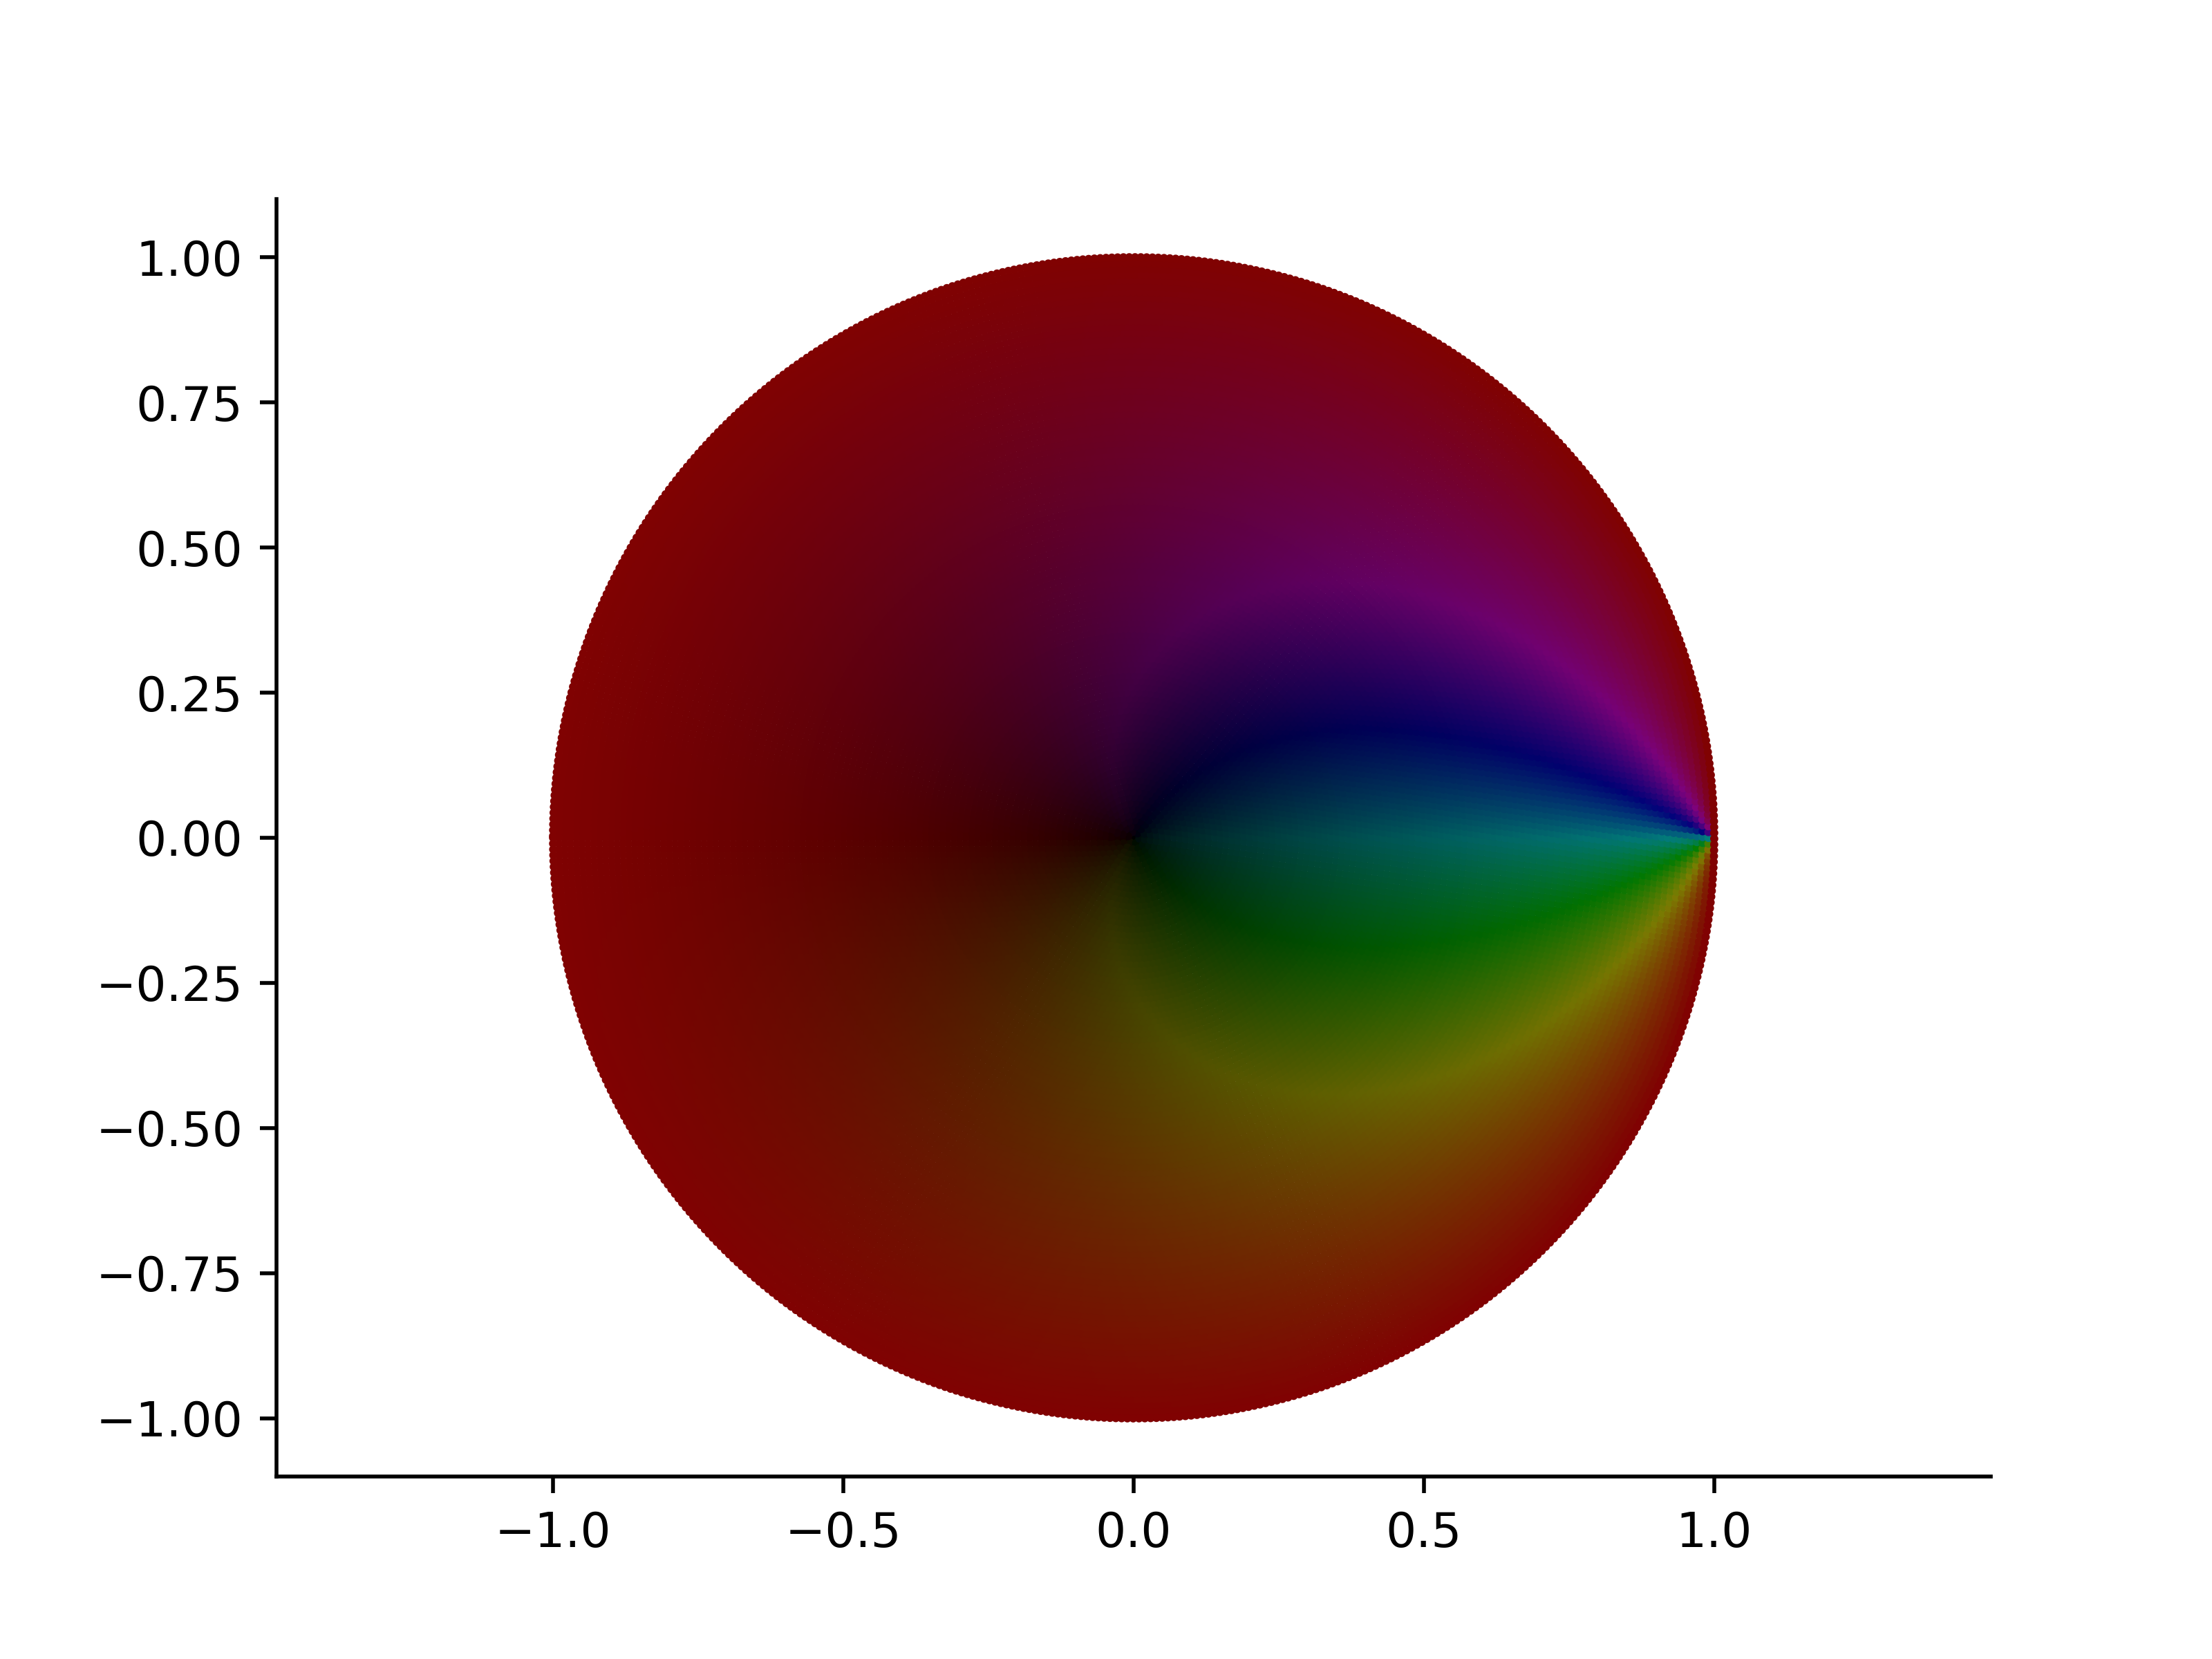
\includegraphics[width=0.7\textwidth]{../Aplicacion/h(z).png}
        \caption{Representación de $-z \frac{\xbar{z} -1}{z - 1}$.}
        \label{fig:h(z)}
    \end{figure}
\end{proof}
